%%% main.tex %%%

%%%%% --------------------------------------------- %%%%%
%	 				  PRÁCTICAS DE						%
%		  TECNOLOGÍAS DE DESARROLLO DE SOFTWARE         %
%														%
%                  JOSÉ SALINAS PARDO                   %
%                 HUGO SÁNCHEZ MARTÍNEZ                 %
%%%%% --------------------------------------------- %%%%%

\documentclass[11pt]{article}

%%% style.tex %%%

%%%%% --------------------------------------------- %%%%%
%	   PACKAGES AND OTHER DOCUMENT CONFIGURATIONS       %
%%%%% --------------------------------------------- %%%%%


\usepackage{amsmath,amsfonts,stmaryrd,amssymb} % Math packages
\usepackage{fancyhdr}
\usepackage{enumerate} % Custom item numbers for enumerations
\usepackage[ruled]{algorithm2e} % Algorithms
\usepackage[framemethod=tikz]{mdframed} % Custom boxed/framed environments

\definecolor{codegray}{gray}{0.925}
\let\colortexttt\texttt
\renewcommand{\texttt}[1]{\colorbox{codegray}{\colortexttt{#1}}}

\usepackage{xcolor} % Colours
\definecolor{mRed}{rgb}{0.8, 0, 0}
\definecolor{mGreen}{rgb}{0,0.6,0}
\definecolor{mGray}{rgb}{0.5,0.5,0.5}
\definecolor{mPurple}{rgb}{0.58,0,0.82}
\definecolor{backgroundColour}{rgb}{0.95,0.95,0.92}

\usepackage{listings} % File listings, with syntax highlighting
\lstset{
	basicstyle=\ttfamily, % Typeset listings in monospace font
	extendedchars=true,  % Soporta caracteres extendidos
	literate={├}{{|-}}1 {─}{{-}}1 {●}{{$\bullet$}}1 {└}{{\texttt{\textbackslash}}}1
}
\lstdefinestyle{PythonStyle}{
	backgroundcolor=\color{backgroundColour},   
	commentstyle=\color{mGreen}\textit,
	keywordstyle=\color{magenta}\bfseries,
	numberstyle=\tiny\color{mGray},
	stringstyle=\color{mPurple},
	basicstyle=\fontfamily{pcr}\selectfont\footnotesize,
	breakatwhitespace=false,         
	breaklines=true,
	captionpos=b,                    
	keepspaces=true,                 
	numbers=left,                    
	numbersep=5pt,
	showspaces=false,                
	showstringspaces=false,
	showtabs=false,                  
	tabsize=2,
	language=Python,
	extendedchars=true,
	inputencoding=utf8
}

\lstdefinestyle{BashStyle}{
	backgroundcolor=\color{lightgray!10},
	keywordstyle=\color{blue!80!black}\bfseries,
	stringstyle=\color{red!70!black},         
	basicstyle=\fontfamily{pcr}\selectfont\small,
	breakatwhitespace=false,
	breaklines=true,
	captionpos=b,
	keepspaces=true,
	numbers=none,                  
	showspaces=false,
	showstringspaces=false,
	showtabs=false,
	tabsize=2,
	language=bash,
	extendedchars=true,
	inputencoding=utf8
}

\lstdefinestyle{TextFileStyle}{
	backgroundcolor=\color{lightgray!5},
	basicstyle=\ttfamily\small,
	numbers=none,
	breaklines=true,
	captionpos=b,
	frame=single,
	rulecolor=\color{gray!30},
	showstringspaces=false,
	tabsize=2,
	language={}
}

\usepackage{colortbl} % Para \arrayrulecolor y colorear tablas
\usepackage{alltt}
\usepackage{array, multirow, tabularx, booktabs} % Tables
\usepackage{float}
\usepackage{tikz}
\usetikzlibrary{quotes,babel, positioning, shapes, shapes.geometric, arrows, calc, external, chains, shadows}
% \usetikzlibrary{arrows.meta, positioning, chains, positioning, shapes.geometric, shadows}
\usepackage{aeguill}
\usepackage{tikzpeople}

\usepackage{pgfplots}

\usepackage[linktoc=none]{hyperref} % para enlaces. linktoc deshabilita indice
\hypersetup{
	colorlinks,
	linkcolor={red}, % footnotes
	urlcolor={blue!80!black}, % urls
	pdftitle={Documentación AppChat},
	pdfsubject={TDS},
	pdfauthor={José Salinas Pardo, Hugo Sánchez Martínez}
}

\usepackage[spanish, es-nodecimaldot]{babel} % Paquete de español

\setlength{\arrayrulewidth}{1.5\arrayrulewidth} % Table rule thickness

% Cambiar título del ToC
\addto\captionsspanish{
	\renewcommand{\contentsname}
	{Contenidos}%
}

\usepackage{listingsutf8}    % Soporte para caracteres UTF-8
\usetikzlibrary{shadows,calc}

\usepackage[inline]{enumitem}   
\makeatletter
% This command ignores the optional argument for itemize and enumerate lists
\newcommand{\inlineitem}[1][]{%
	\ifnum\enit@type=\tw@
	{\descriptionlabel{#1}}
	\hspace{\labelsep}%
	\else
	\ifnum\enit@type=\z@
	\refstepcounter{\@listctr}\fi
	\quad\@itemlabel\hspace{\labelsep}%
	\fi}
\makeatother
\parindent=0pt

% some parameters for customization
\def\shadowshift{3pt,-3pt}
\def\shadowradius{6pt}

\colorlet{innercolor}{black!50}
\colorlet{outercolor}{gray!05}

% this draws a shadow under a rectangle node
\newcommand\drawshadow[1]{
	\begin{pgfonlayer}{shadow}
		\shade[outercolor,inner color=innercolor,outer color=outercolor] ($(#1.south west)+(\shadowshift)+(\shadowradius/2,\shadowradius/2)$) circle (\shadowradius);
		\shade[outercolor,inner color=innercolor,outer color=outercolor] ($(#1.north west)+(\shadowshift)+(\shadowradius/2,-\shadowradius/2)$) circle (\shadowradius);
		\shade[outercolor,inner color=innercolor,outer color=outercolor] ($(#1.south east)+(\shadowshift)+(-\shadowradius/2,\shadowradius/2)$) circle (\shadowradius);
		\shade[outercolor,inner color=innercolor,outer color=outercolor] ($(#1.north east)+(\shadowshift)+(-\shadowradius/2,-\shadowradius/2)$) circle (\shadowradius);
		\shade[top color=innercolor,bottom color=outercolor] ($(#1.south west)+(\shadowshift)+(\shadowradius/2,-\shadowradius/2)$) rectangle ($(#1.south east)+(\shadowshift)+(-\shadowradius/2,\shadowradius/2)$);
		\shade[left color=innercolor,right color=outercolor] ($(#1.south east)+(\shadowshift)+(-\shadowradius/2,\shadowradius/2)$) rectangle ($(#1.north east)+(\shadowshift)+(\shadowradius/2,-\shadowradius/2)$);
		\shade[bottom color=innercolor,top color=outercolor] ($(#1.north west)+(\shadowshift)+(\shadowradius/2,-\shadowradius/2)$) rectangle ($(#1.north east)+(\shadowshift)+(-\shadowradius/2,\shadowradius/2)$);
		\shade[outercolor,right color=innercolor,left color=outercolor] ($(#1.south west)+(\shadowshift)+(-\shadowradius/2,\shadowradius/2)$) rectangle ($(#1.north west)+(\shadowshift)+(\shadowradius/2,-\shadowradius/2)$);
		\filldraw ($(#1.south west)+(\shadowshift)+(\shadowradius/2,\shadowradius/2)$) rectangle ($(#1.north east)+(\shadowshift)-(\shadowradius/2,\shadowradius/2)$);
	\end{pgfonlayer}
}

% create a shadow layer, so that we don't need to worry about overdrawing other things
\pgfdeclarelayer{shadow} 
\pgfsetlayers{shadow,main}

\newsavebox\mybox
\newlength\mylen

\newcommand\shadowimage[2][]{%
	\setbox0=\hbox{\includegraphics[#1]{#2}}
	\setlength\mylen{\wd0}
	\ifnum\mylen<\ht0
	\setlength\mylen{\ht0}
	\fi
	\divide \mylen by 120
	\def\shadowshift{\mylen,-\mylen}
	\def\shadowradius{\the\dimexpr\mylen+\mylen+\mylen\relax}
	\begin{tikzpicture}
		\node[anchor=south west,inner sep=0] (image) at (0,0) {\includegraphics[#1]{#2}};
		\drawshadow{image}
\end{tikzpicture}}

\renewcommand{\footnoterule}{%
	\vspace{1cm} % Espacio adicional antes de la línea
	\hrule width 0.8\textwidth % Ajusta el ancho de la línea (80% del ancho del texto)
	\vspace{2cm} % Espacio adicional después de la línea
}


%%%%% --------------------------------------------- %%%%%
%	                 DOCUMENT MARGINS
%%%%% --------------------------------------------- %%%%%

\usepackage{geometry} % Required for adjusting page dimensions and margins

\geometry{
	a4paper, % Papaer size
	margin={2cm,3cm},
	headheight=14pt, % Header height
	footskip=1cm, % Space from the bottom margin to the baseline of the footer
	headsep=1.2cm, % Space from the top margin to the baseline of the header
	%showframe, % Uncomment to show how the type block is set on the page
}

%%%%% --------------------------------------------- %%%%%
%	                      FONTS                         %
%%%%% --------------------------------------------- %%%%%

\usepackage[utf8]{inputenc} % Required for inputting international characters
\usepackage[T1]{fontenc} % Output font encoding for international characters
\usepackage[
protrusion=true,
activate={true,nocompatibility},
final,
tracking=true,
kerning=true,
spacing=true,
factor=1100]{microtype}
\SetTracking{encoding={*}, shape=sc}{40}


% Choose font:
\usepackage{mathptmx} 	 % Times
% \usepackage{mathpazo}  % Palatino
% \usepackage{lmodern}	 % Upgraded LaTeX font

%%%%% --------------------------------------------- %%%%%
%	            COMMAND LINE ENVIRONMENT                %
%%%%% --------------------------------------------- %%%%%

% Usage:
% \begin{commandline}
	%	\begin{verbatim}
		%		$ ls
		%		
		%		Applications	Desktop	...
		%	\end{verbatim}
	% \end{commandline}

\mdfdefinestyle{commandline}{
	leftmargin=10pt,
	rightmargin=10pt,
	innerleftmargin=15pt,
	middlelinecolor=black!50!white,
	middlelinewidth=2pt,
	frametitlerule=false,
	backgroundcolor=black!5!white,
	frametitle={Bash},
	frametitlefont={\normalfont\sffamily\color{white}\hspace{-1em}},
	frametitlebackgroundcolor=black!50!white,
	nobreak,
}

% Define a custom environment for command-line snapshots
\newenvironment{commandline}{
	\medskip
	\begin{mdframed}[style=commandline]
	}{
	\end{mdframed}
	\medskip
}

%%%%% --------------------------------------------- %%%%%
%	             FILE CONTENTS ENVIRONMENT              %
%%%%% --------------------------------------------- %%%%%

% Usage:
% \begin{file}[optional filename, defaults to "File"]
	%	File contents, for example, with a listings environment
	% \end{file}

\mdfdefinestyle{file}{
	innertopmargin=1.6\baselineskip,
	innerbottommargin=0.8\baselineskip,
	innerleftmargin=1.6\baselineskip,
	topline=false, bottomline=false,
	leftline=false, rightline=false,
	leftmargin=2cm,
	rightmargin=2cm,
	singleextra={%
		\draw[fill=black!10!white](P)++(0,-1.2em)rectangle(P-|O);
		\node[anchor=north west]
		at(P-|O){\ttfamily\mdfilename};
		%
		\def\l{3em}
		\draw(O-|P)++(-\l,0)--++(\l,\l)--(P)--(P-|O)--(O)--cycle;
		\draw(O-|P)++(-\l,0)--++(0,\l)--++(\l,0);
	},
	nobreak,
}

% Define a custom environment for file contents
\newenvironment{file}[1][File]{ % Set the default filename to "File"
	\medskip
	\newcommand{\mdfilename}{#1}
	\begin{mdframed}[style=file]
	}{
	\end{mdframed}
	\medskip
}

%%%%% --------------------------------------------- %%%%%
%	          NUMBERED QUESTIONS ENVIRONMENT            %
%%%%% --------------------------------------------- %%%%%

% Usage:
% \begin{question}[optional title]
	%	Question contents
	% \end{question}

\mdfdefinestyle{question}{
	innertopmargin=1.2\baselineskip,
	innerbottommargin=0.8\baselineskip,
	roundcorner=5pt,
	nobreak,
	singleextra={%
		\draw(P-|O)node[xshift=1em,anchor=west,fill=white,draw,rounded corners=5pt]{%
			Question \theQuestion\questionTitle};
	},
}

\newcounter{Question} % Stores the current question number that gets iterated with each new question

% Define a custom environment for numbered questions
\newenvironment{question}[1][\unskip]{
	\bigskip
	\stepcounter{Question}
	\newcommand{\questionTitle}{~#1}
	\begin{mdframed}[style=question]
	}{
	\end{mdframed}
	\medskip
}


%%%%% --------------------------------------------- %%%%%
%	              WARNING TEXT ENVIRONMENT              %
%%%%% --------------------------------------------- %%%%%

% Usage:
% \begin{warn}[optional title, defaults to "Warning:"]
	%	Contents
	% \end{warn}

\mdfdefinestyle{warning}{
	topline=false, bottomline=false,
	leftline=false, rightline=false,
	nobreak,
	singleextra={%
		\draw(P-|O)++(-0.5em,0)node(tmp1){};
		\draw(P-|O)++(0.5em,0)node(tmp2){};
		\fill[black,rotate around={45:(P-|O)}](tmp1)rectangle(tmp2);
		\node at(P-|O){\color{white}\scriptsize\bf !};
		\draw[very thick](P-|O)++(0,-1em)--(O);%--(O-|P);
	}
}

% Define a custom environment for warning text
\newenvironment{warn}[1][Warning:]{ % Set the default warning to "Warning:"
	\medskip
	\begin{mdframed}[style=warning]
		\noindent{\textbf{#1}}
	}{
	\end{mdframed}
}


%%%%% --------------------------------------------- %%%%%
%                 INFORMATION ENVIRONMENT               %
%%%%% --------------------------------------------- %%%%%

% Usage:
% \begin{info}[optional title, defaults to "Info:"]
	% 	contents
	% 	\end{info}

\mdfdefinestyle{info}{%
	topline=false, bottomline=false,
	leftline=false, rightline=false,
	nobreak,
	singleextra={%
		\fill[black](P-|O)circle[radius=0.4em];
		\node at(P-|O){\color{white}\scriptsize\bf i};
		\draw[very thick](P-|O)++(0,-0.8em)--(O);%--(O-|P);
	}
}

% Define a custom environment for information
\newenvironment{info}[1][Info:]{ % Set the default title to "Info:"
	\medskip
	\begin{mdframed}[style=info]
		\noindent{\textbf{#1}}
	}{
	\end{mdframed}
}



\begin{document}

\title{
	\vspace{-5ex}
	\begin{figure}[H]
		\centering
		
\includegraphics[width=72mm]{umu-logo.pdf}
	\end{figure}
	
	{\Large \textsc{Universidad de Murcia}}\\
	{\Large Facultad de Informática}\\ [12.5ex]
	{\Large \textsc{Prácticas de}\\ [1ex]}
	{\Huge Tecnologías de Desarrollo de Software}\\ [1ex]
	{\Large \textsc{3º de Grado en Ingeniería Informática}}\\
	{\Large \textsc{Profesor: }} \\
	{\Large \textsc{Grupo 2.3}} \\
	{\Large \textsc{Curso 2024/2025}} \\ 
	\vspace{10ex}
}

\author{
	{\Large José Salinas Pardo}\\[0.5ex]
	48740555J\\
	\texttt{j.salinaspardo@um.es}
	\and
	{\Large Hugo Sánchez Martínez}\\[0.5ex]
	24450997L\\
	\texttt{hugo.s.m@um.es}\\
}

\pagestyle{fancy}
\fancyhf{}
\fancyhead[LE]{\nouppercase{\rightmark} \hfill \textbf{\nouppercase{\leftmark}}}   % Encabezado en la página izquierda (even) sin mayúsculas
\fancyhead[RO]{\nouppercase{\rightmark}}  % Encabezado en la página derecha (odd) sin mayúsculas
\setlength{\headheight}{25pt}  % Ajusta la altura del encabezado
\fancyfoot[R]{J. Salinas, H. Sánchez}
\fancyfoot[C]{\thepage}

\date{\vspace{-10ex}}
\maketitle
\thispagestyle{empty} % Elimina el número de página de la portada
\clearpage

\thispagestyle{empty} % Elimina el número de página del ToC
\tableofcontents
\clearpage
\thispagestyle{empty} % Elimina el número de página del ToC
\listoffigures
\clearpage
\setcounter{page}{1}



\thispagestyle{empty}

\hrule
\vspace{-5.4ex}
\begin{abstract}
\vspace{1ex}
Este documento especifica la implementación de las prácticas de la asignatura Tecnologías de Desarrollo de Software del tercer curso del grado en Ingeniería Informática de la Universidad de Murcia.\\

Dicha práctica consiste en el desarrollo de una aplicación de mensajería (\textit{chatting}), \textbf{AppChat}, basada en aplicaciones ya existentes. El objetivo de este documento es describir en detalle el proceso de desarrollo de la aplicación, desde la planificación inicial y el análisis de requisitos, hasta la implementación y las pruebas finales.
\vspace{0.5ex}
\end{abstract}
\hrule
\vspace{4ex}

\section{Introducción}

\textbf{AppChat} es una aplicación de escritorio de mensajería instantánea desarrollada en Java 8. Basada en soluciones reales como \textit{Telegram} o \textit{Whatsapp}, AppChat permite a los usuarios llevar una gestión simple de sus contactos, ofreciendo la posibilidad de crear grupos y enviar mensajes como si fuesen ``\textit{grupos de difusión}''.

\section{Requisitos}

AppChat requiere al menos tener instalada al menos la versión 8 de \href{https://www.oracle.com/java/technologies/javase/javase8-archive-downloads.html}{Java SE} para ejecutar.

\section{Tecnologías}

Durante el desarrollo de AppChat se han usado las siguientes tecnologías:

\begin{itemize}
	\item \textbf{Git}: Para el control de versiones y colaboración en el desarrollo.
	\item \textbf{Maven}: Utilizado como herramienta de gestión y construcción del proyecto.
	\item \textbf{Eclipse}: Se ha escodigo Eclipse como entorno de desarrollo (IDE).
	\item \textbf{PlantUML}: Usado para generar los diagramas UML del modelo.
	\item \textbf{Java Swing}: Biblioteca gráfica empleada para el desarrollo de la interfaz de usuario.
\end{itemize}

\clearpage

\section{Requisitos y Modelado de Clases}

\subsection{\textit{User Story Mapping}}

Realizamos una \textbf{representación visual} de las funcionalidades de la aplicación desde la perspectiva de usuario. El eje horizontal representa el flujo de trabajo de un usuario en un orden lógico, mientras que el eje vertical organiza las historias en función de su importancia.

\begin{figure}[h]
    \centering
    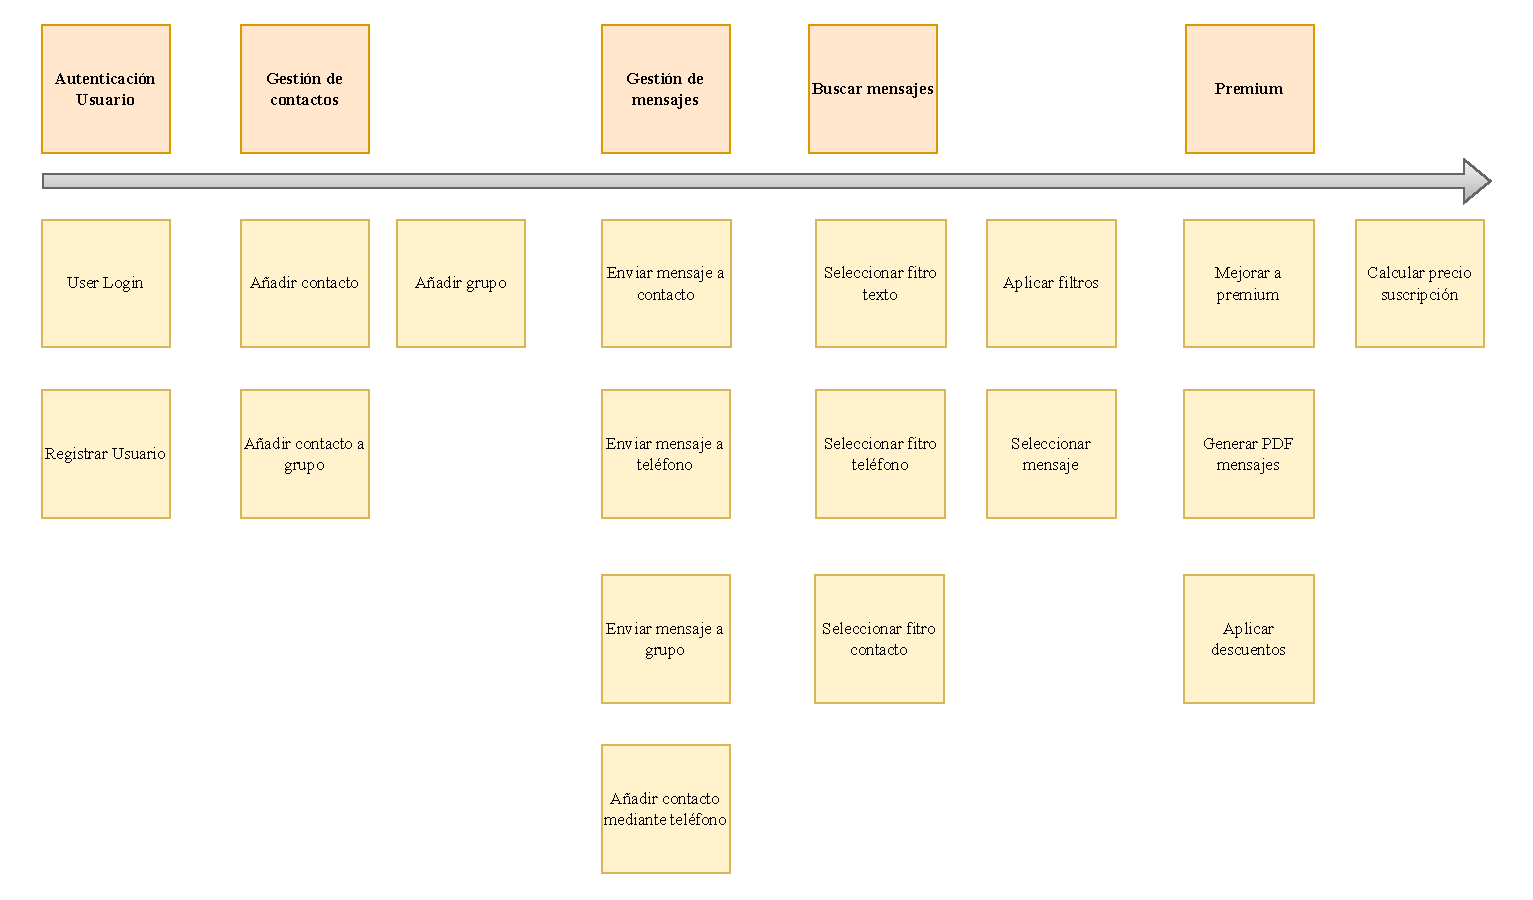
\includegraphics[width=\linewidth]{user-story-mapping.drawio-2.pdf}
    \caption{Diagrama de historias de usuario de AppChat}
    \label{fig:user-story-mapping}
\end{figure}

\subsection{Diagrama de clases}

\begin{figure}[H]
	\centering
	\scalebox{0.425}{
		% generated by Plantuml 1.2020.02      
\definecolor{plantucolor0000}{RGB}{238,232,170}
\definecolor{plantucolor0001}{RGB}{0,0,0}
\definecolor{plantucolor0002}{RGB}{180,167,229}
\definecolor{plantucolor0003}{RGB}{132,190,132}
\definecolor{plantucolor0004}{RGB}{3,128,72}
\definecolor{plantucolor0005}{RGB}{173,209,178}
\definecolor{plantucolor0006}{RGB}{255,255,0}
\definecolor{plantucolor0007}{RGB}{168,0,54}
\definecolor{plantucolor0008}{RGB}{200,41,48}
\definecolor{plantucolor0009}{RGB}{169,220,223}
\definecolor{plantucolor0010}{RGB}{242,77,92}
\definecolor{plantucolor0011}{RGB}{255,255,255}
\begin{tikzpicture}[yscale=-1
	,pstyle0/.style={color=black,fill=plantucolor0000,line width=1.0pt}
	,pstyle1/.style={color=black,fill=plantucolor0002,line width=1.0pt}
	,pstyle2/.style={color=black,line width=1.0pt}
	,pstyle3/.style={color=plantucolor0004,fill=plantucolor0003,line width=1.0pt}
	,pstyle4/.style={color=black,fill=plantucolor0005,line width=1.0pt}
	,pstyle5/.style={color=plantucolor0007,fill=plantucolor0006,line width=1.0pt}
	,pstyle6/.style={color=plantucolor0008,line width=1.0pt}
	,pstyle9/.style={color=plantucolor0007,line width=1.0pt,dash pattern=on 7.0pt off 7.0pt}
	,pstyle10/.style={color=plantucolor0007,line width=1.0pt}
	,pstyle11/.style={color=plantucolor0007,fill=plantucolor0007,line width=1.0pt}
	,pstyle12/.style={color=plantucolor0007,fill=white,line width=1.0pt}
	]
	\draw[pstyle0] (87.5pt,104.5pt) arc (180:270:10pt) -- (97.5pt,94.5pt) -- (214.1204pt,94.5pt) arc (270:360:10pt) -- (224.1204pt,104.5pt) -- (224.1204pt,139.4819pt) arc (0:90:10pt) -- (214.1204pt,149.4819pt) -- (97.5pt,149.4819pt) arc (90:180:10pt) -- (87.5pt,139.4819pt) -- cycle;
	\draw[pstyle1] (117.613pt,110.5pt) ellipse (11pt and 11pt);
	\node at (117.613pt,110.5pt)[]{\textbf{\Large I}};
	\node at (134.9714pt,102.3279pt)[below right,color=black]{\textit{\textbf{Descuento}}};
	\draw[pstyle2] (88.5pt,126.5pt) -- (223.1204pt,126.5pt);
	\draw[pstyle3] (98.5pt,137.5pt) ellipse (3pt and 3pt);
	\node at (107.5pt,130.5pt)[below right,color=black]{aplicarDescuento()};
	\draw[pstyle0] (6pt,256pt) arc (180:270:10pt) -- (16pt,246pt) -- (45.7pt,246pt) arc (270:360:10pt) -- (55.7pt,256pt) -- (55.7pt,268pt) arc (0:90:10pt) -- (45.7pt,278pt) -- (16pt,278pt) arc (90:180:10pt) -- (6pt,268pt) -- cycle;
	\draw[pstyle4] (21pt,262pt) ellipse (11pt and 11pt);
	\node at (21pt,262pt)[]{\textbf{\Large C}};
	\node at (35pt,253.8279pt)[below right,color=black]{\textbf{D1}};
	\draw[pstyle0] (131pt,256pt) arc (180:270:10pt) -- (141pt,246pt) -- (170.7pt,246pt) arc (270:360:10pt) -- (180.7pt,256pt) -- (180.7pt,268pt) arc (0:90:10pt) -- (170.7pt,278pt) -- (141pt,278pt) arc (90:180:10pt) -- (131pt,268pt) -- cycle;
	\draw[pstyle4] (146pt,262pt) ellipse (11pt and 11pt);
	\node at (146pt,262pt)[]{\textbf{\Large C}};
	\node at (160pt,253.8279pt)[below right,color=black]{\textbf{D2}};
	\draw[pstyle0] (489.5pt,104.5pt) arc (180:270:10pt) -- (499.5pt,94.5pt) -- (570.5717pt,94.5pt) arc (270:360:10pt) -- (580.5717pt,104.5pt) -- (580.5717pt,139.4819pt) arc (0:90:10pt) -- (570.5717pt,149.4819pt) -- (499.5pt,149.4819pt) arc (90:180:10pt) -- (489.5pt,139.4819pt) -- cycle;
	\draw[pstyle4] (504.5pt,110.5pt) ellipse (11pt and 11pt);
	\node at (504.5pt,110.5pt)[]{\textbf{\Large C}};
	\node at (518.5pt,102.3279pt)[below right,color=black]{\textbf{AppChat}};
	\draw[pstyle2] (490.5pt,126.5pt) -- (579.5717pt,126.5pt);
	\draw[pstyle3] (500.5pt,137.5pt) ellipse (3pt and 3pt);
	\node at (509.5pt,130.5pt)[below right,color=black]{login()};
	\draw[pstyle5] (481pt,13pt) -- (481pt,30.706pt) -- (531pt,35.706pt) -- (535pt,94.36pt) -- (539pt,35.706pt) -- (584.4105pt,35.706pt) -- (589.4105pt,18pt) -- (579.4105pt,8pt) -- (486pt,8pt);
	\draw[pstyle5] (579.4105pt,8pt) -- (579.4105pt,15.5pt) -- (589.4105pt,18pt) -- (579.4105pt,8pt);
	\node at (487pt,13pt)[below right,color=black]{Controlador};
	\draw[pstyle0] (655.5pt,97pt) arc (180:270:10pt) -- (665.5pt,87pt) -- (818.3918pt,87pt) arc (270:360:10pt) -- (828.3918pt,97pt) -- (828.3918pt,146.9638pt) arc (0:90:10pt) -- (818.3918pt,156.9638pt) -- (665.5pt,156.9638pt) arc (90:180:10pt) -- (655.5pt,146.9638pt) -- cycle;
	\draw[pstyle4] (670.5pt,103pt) ellipse (11pt and 11pt);
	\node at (670.5pt,103pt)[]{\textbf{\Large C}};
	\node at (684.5pt,94.8279pt)[below right,color=black]{\textbf{RepositorioUsuarios}};
	\draw[pstyle2] (656.5pt,119pt) -- (827.3918pt,119pt);
	\draw[pstyle3] (666.5pt,130pt) ellipse (3pt and 3pt);
	\node at (675.5pt,123pt)[below right,color=black]{getUsuario()};
	\draw[pstyle3] (666.5pt,144.9819pt) ellipse (3pt and 3pt);
	\node at (675.5pt,137.9819pt)[below right,color=black]{addUsuario()};
	\draw[pstyle0] (674.5pt,218pt) arc (180:270:10pt) -- (684.5pt,208pt) -- (799.7pt,208pt) arc (270:360:10pt) -- (809.7pt,218pt) -- (809.7pt,305.9276pt) arc (0:90:10pt) -- (799.7pt,315.9276pt) -- (684.5pt,315.9276pt) arc (90:180:10pt) -- (674.5pt,305.9276pt) -- cycle;
	\draw[pstyle4] (711.594pt,224pt) ellipse (11pt and 11pt);
	\node at (711.594pt,224pt)[]{\textbf{\Large C}};
	\node at (730.5038pt,215.8279pt)[below right,color=black]{\textbf{Usuario}};
	\draw[pstyle2] (675.5pt,240pt) -- (808.7pt,240pt);
	\draw[pstyle6] (682.5pt,248pt) rectangle (688.5pt,254pt);
	\node at (694.5pt,244pt)[below right,color=black]{nombre: String};
	\draw[pstyle6] (682.5pt,262.9819pt) rectangle (688.5pt,268.9819pt);
	\node at (694.5pt,258.9819pt)[below right,color=black]{email: String};
	\draw[pstyle6] (682.5pt,277.9638pt) rectangle (688.5pt,283.9638pt);
	\node at (694.5pt,273.9638pt)[below right,color=black]{telefono: String};
	\draw[pstyle6] (682.5pt,292.9457pt) rectangle (688.5pt,298.9457pt);
	\node at (694.5pt,288.9457pt)[below right,color=black]{premium: Boolean};
	\draw[pstyle2] (675.5pt,307.9276pt) -- (808.7pt,307.9276pt);
	\draw[pstyle0] (680.5pt,384.5pt) arc (180:270:10pt) -- (690.5pt,374.5pt) -- (785.2241pt,374.5pt) arc (270:360:10pt) -- (795.2241pt,384.5pt) -- (795.2241pt,427.4819pt) arc (0:90:10pt) -- (785.2241pt,437.4819pt) -- (690.5pt,437.4819pt) arc (90:180:10pt) -- (680.5pt,427.4819pt) -- cycle;
	\draw[color=black,fill=plantucolor0009,line width=1.0pt] (704.4658pt,390.5pt) ellipse (11pt and 11pt);
	\node at (704.4658pt,390.5pt)[]{\textbf{\Large A}};
	\node at (720.4582pt,382.3279pt)[below right,color=black]{\textit{\textbf{Contacto}}};
	\draw[pstyle2] (681.5pt,406.5pt) -- (794.2241pt,406.5pt);
	\draw[pstyle6] (688.5pt,414.5pt) rectangle (694.5pt,420.5pt);
	\node at (700.5pt,410.5pt)[below right,color=black]{nombre: String};
	\draw[pstyle2] (681.5pt,429.4819pt) -- (794.2241pt,429.4819pt);
	\draw[pstyle0] (550.5pt,524pt) arc (180:270:10pt) -- (560.5pt,514pt) -- (673.2828pt,514pt) arc (270:360:10pt) -- (683.2828pt,524pt) -- (683.2828pt,581.9638pt) arc (0:90:10pt) -- (673.2828pt,591.9638pt) -- (560.5pt,591.9638pt) arc (90:180:10pt) -- (550.5pt,581.9638pt) -- cycle;
	\draw[pstyle4] (591.327pt,530pt) ellipse (11pt and 11pt);
	\node at (591.327pt,530pt)[]{\textbf{\Large C}};
	\node at (611.0663pt,521.8279pt)[below right,color=black]{\textbf{Grupo}};
	\draw[pstyle2] (551.5pt,546pt) -- (682.2828pt,546pt);
	\draw[pstyle6] (558.5pt,554pt) rectangle (564.5pt,560pt);
	\node at (570.5pt,550pt)[below right,color=black]{nombre: String};
	\draw[pstyle2] (551.5pt,568.9819pt) -- (682.2828pt,568.9819pt);
	\draw[color=plantucolor0008,fill=plantucolor0010,line width=1.0pt] (558.5pt,576.9819pt) rectangle (564.5pt,582.9819pt);
	\node at (570.5pt,572.9819pt)[below right,color=black]{agregarContacto()};
	\draw[pstyle0] (870.5pt,377pt) arc (180:270:10pt) -- (880.5pt,367pt) -- (983.9667pt,367pt) arc (270:360:10pt) -- (993.9667pt,377pt) -- (993.9667pt,434.9638pt) arc (0:90:10pt) -- (983.9667pt,444.9638pt) -- (880.5pt,444.9638pt) arc (90:180:10pt) -- (870.5pt,434.9638pt) -- cycle;
	\draw[pstyle4] (901.1pt,383pt) ellipse (11pt and 11pt);
	\node at (901.1pt,383pt)[]{\textbf{\Large C}};
	\node at (918.5667pt,374.8279pt)[below right,color=black]{\textbf{Mensaje}};
	\draw[pstyle2] (871.5pt,399pt) -- (992.9667pt,399pt);
	\draw[pstyle6] (878.5pt,407pt) rectangle (884.5pt,413pt);
	\node at (890.5pt,403pt)[below right,color=black]{texto: String};
	\draw[pstyle6] (878.5pt,421.9819pt) rectangle (884.5pt,427.9819pt);
	\node at (890.5pt,417.9819pt)[below right,color=black]{fechaHora: Date};
	\draw[pstyle2] (871.5pt,436.9638pt) -- (992.9667pt,436.9638pt);
	\draw[pstyle0] (759pt,524pt) arc (180:270:10pt) -- (769pt,514pt) -- (913.3724pt,514pt) arc (270:360:10pt) -- (923.3724pt,524pt) -- (923.3724pt,581.9638pt) arc (0:90:10pt) -- (913.3724pt,591.9638pt) -- (769pt,591.9638pt) arc (90:180:10pt) -- (759pt,581.9638pt) -- cycle;
	\draw[pstyle4] (774pt,530pt) ellipse (11pt and 11pt);
	\node at (774pt,530pt)[]{\textbf{\Large C}};
	\node at (788pt,521.8279pt)[below right,color=black]{\textbf{ContactoIndividual}};
	\draw[pstyle2] (760pt,546pt) -- (922.3724pt,546pt);
	\draw[pstyle6] (767pt,554pt) rectangle (773pt,560pt);
	\node at (779pt,550pt)[below right,color=black]{telefono : String};
	\draw[pstyle6] (767pt,568.9819pt) rectangle (773pt,574.9819pt);
	\node at (779pt,564.9819pt)[below right,color=black]{usuario : Usuario};
	\draw[pstyle2] (760pt,583.9638pt) -- (922.3724pt,583.9638pt);
	\draw[pstyle0] (462.5pt,244.5pt) arc (180:270:10pt) -- (472.5pt,234.5pt) -- (589.1204pt,234.5pt) arc (270:360:10pt) -- (599.1204pt,244.5pt) -- (599.1204pt,279.4819pt) arc (0:90:10pt) -- (589.1204pt,289.4819pt) -- (472.5pt,289.4819pt) arc (90:180:10pt) -- (462.5pt,279.4819pt) -- cycle;
	\draw[pstyle1] (506.4839pt,250.5pt) ellipse (11pt and 11pt);
	\node at (506.4839pt,250.5pt)[]{\textbf{\Large I}};
	\node at (526.9248pt,242.3279pt)[below right,color=black]{\textit{\textbf{Filtro}}};
	\draw[pstyle2] (463.5pt,266.5pt) -- (598.1204pt,266.5pt);
	\draw[pstyle3] (473.5pt,277.5pt) ellipse (3pt and 3pt);
	\node at (482.5pt,270.5pt)[below right,color=black]{aplicarDescuento()};
	\draw[pstyle0] (283pt,400pt) arc (180:270:10pt) -- (293pt,390pt) -- (383.3647pt,390pt) arc (270:360:10pt) -- (393.3647pt,400pt) -- (393.3647pt,412pt) arc (0:90:10pt) -- (383.3647pt,422pt) -- (293pt,422pt) arc (90:180:10pt) -- (283pt,412pt) -- cycle;
	\draw[pstyle4] (298pt,406pt) ellipse (11pt and 11pt);
	\node at (298pt,406pt)[]{\textbf{\Large C}};
	\node at (312pt,397.8279pt)[below right,color=black]{\textbf{FiltroTexto}};
	\draw[pstyle0] (256.5pt,256pt) arc (180:270:10pt) -- (266.5pt,246pt) -- (377.9791pt,246pt) arc (270:360:10pt) -- (387.9791pt,256pt) -- (387.9791pt,268pt) arc (0:90:10pt) -- (377.9791pt,278pt) -- (266.5pt,278pt) arc (90:180:10pt) -- (256.5pt,268pt) -- cycle;
	\draw[pstyle4] (271.5pt,262pt) ellipse (11pt and 11pt);
	\node at (271.5pt,262pt)[]{\textbf{\Large C}};
	\node at (285.5pt,253.8279pt)[below right,color=black]{\textbf{FiltroContacto}};
	\draw[pstyle0] (468.5pt,400pt) arc (180:270:10pt) -- (478.5pt,390pt) -- (589.514pt,390pt) arc (270:360:10pt) -- (599.514pt,400pt) -- (599.514pt,412pt) arc (0:90:10pt) -- (589.514pt,422pt) -- (478.5pt,422pt) arc (90:180:10pt) -- (468.5pt,412pt) -- cycle;
	\draw[pstyle4] (483.5pt,406pt) ellipse (11pt and 11pt);
	\node at (483.5pt,406pt)[]{\textbf{\Large C}};
	\node at (497.5pt,397.8279pt)[below right,color=black]{\textbf{FiltroTelefono}};
	\draw[pstyle9] (118.45pt,164.45pt) ..controls (93.49pt,192.01pt) and (62.18pt,226.58pt) .. (44.6pt,245.99pt);
	\draw[pstyle10] (113.28pt,159.73pt) -- (131.9pt,149.61pt) -- (123.66pt,169.13pt) -- (113.28pt,159.73pt) -- cycle;
	\draw[pstyle9] (156pt,169.92pt) ..controls (156pt,196.45pt) and (156pt,227.84pt) .. (156pt,245.99pt);
	\draw[pstyle10] (149pt,169.61pt) -- (156pt,149.61pt) -- (163pt,169.61pt) -- (149pt,169.61pt) -- cycle;
	\draw[pstyle10] (230.01pt,122pt) ..controls (316.43pt,122pt) and (402.84pt,122pt) .. (489.26pt,122pt);
	\draw[pstyle11] (224.84pt,122pt) -- (233.84pt,126pt) -- (229.84pt,122pt) -- (233.84pt,118pt) -- (224.84pt,122pt) -- cycle;
	\draw[pstyle10] (593.81pt,122pt) ..controls (614.33pt,122pt) and (634.84pt,122pt) .. (655.36pt,122pt);
	\draw[pstyle11] (580.69pt,122pt) -- (586.69pt,126pt) -- (592.69pt,122pt) -- (586.69pt,118pt) -- (580.69pt,122pt) -- cycle;
	\node at (639.0275pt,104.2506pt)[below right,color=black]{1};
	\draw[pstyle10] (742pt,170.29pt) ..controls (742pt,182.42pt) and (742pt,195.54pt) .. (742pt,207.94pt);
	\draw[pstyle12] (742pt,157.11pt) -- (738pt,163.11pt) -- (742pt,169.11pt) -- (746pt,163.11pt) -- (742pt,157.11pt) -- cycle;
	\node at (717.3828pt,182.1972pt)[below right,color=black]{0..*};
	\draw[pstyle10] (574.91pt,149.61pt) ..controls (602.99pt,168.33pt) and (641.26pt,193.84pt) .. (674.1pt,215.73pt);
	\node at (658.2469pt,192.7821pt)[below right,color=black]{1};
	\draw[pstyle10] (740.13pt,329.29pt) ..controls (739.69pt,344.95pt) and (739.24pt,360.92pt) .. (738.87pt,374.13pt);
	\draw[pstyle12] (740.5pt,316.28pt) -- (736.3367pt,322.1679pt) -- (740.1705pt,328.2755pt) -- (744.3337pt,322.3876pt) -- (740.5pt,316.28pt) -- cycle;
	\node at (731.8419pt,323.9788pt)[below right,color=black]{1};
	\node at (731.4415pt,348.8784pt)[below right,color=black]{*};
	\draw[pstyle10] (699.36pt,453.3pt) ..controls (683.08pt,472.82pt) and (664.35pt,495.26pt) .. (648.88pt,513.8pt);
	\draw[pstyle10] (694.15pt,448.62pt) -- (712.34pt,437.75pt) -- (704.9pt,457.59pt) -- (694.15pt,448.62pt) -- cycle;
	\node at (685pt,471pt)[below right,color=black]{\guillemotleft extends\guillemotright };
	\draw[pstyle10] (771.52pt,454.18pt) ..controls (785.23pt,473.49pt) and (800.89pt,495.53pt) .. (813.87pt,513.8pt);
	\draw[pstyle10] (765.72pt,458.11pt) -- (759.84pt,437.75pt) -- (777.13pt,450pt) -- (765.72pt,458.11pt) -- cycle;
	\node at (796pt,471pt)[below right,color=black]{\guillemotleft extends\guillemotright };
	\draw[pstyle10] (795.59pt,406pt) ..controls (820.55pt,406pt) and (845.5pt,406pt) .. (870.46pt,406pt);
	\node at (802.3645pt,388.2317pt)[below right,color=black]{receptor};
	\node at (797.3688pt,406.7624pt)[below right,color=black]{recibidos};
	\draw[pstyle10] (809.52pt,313.46pt) ..controls (833.09pt,331.08pt) and (859.14pt,350.54pt) .. (881.12pt,366.98pt);
	\node at (817.723pt,300.3208pt)[below right,color=black]{emisor};
	\node at (779.4904pt,341.3159pt)[below right,color=black]{enviados 0..*};
	\draw[pstyle10] (697.09pt,553pt) ..controls (717.66pt,553pt) and (738.22pt,553pt) .. (758.79pt,553pt);
	\draw[pstyle12] (683.94pt,553pt) -- (689.94pt,557pt) -- (695.94pt,553pt) -- (689.94pt,549pt) -- (683.94pt,553pt) -- cycle;
	\node at (727.7294pt,535.3014pt)[below right,color=black]{0..*};
	\draw[pstyle9] (478.34pt,301.75pt) ..controls (438.76pt,330.87pt) and (386.69pt,369.18pt) .. (358.41pt,389.98pt);
	\draw[pstyle10] (474.44pt,295.92pt) -- (494.7pt,289.71pt) -- (482.74pt,307.2pt) -- (474.44pt,295.92pt) -- cycle;
	\draw[pstyle9] (387.72pt,262pt) ..controls (405.91pt,262pt) and (424.11pt,262pt) .. (442.3pt,262pt);
	\draw[pstyle10] (442.44pt,255pt) -- (462.44pt,262pt) -- (442.44pt,269pt) -- (442.44pt,255pt) -- cycle;
	\draw[pstyle9] (531.99pt,309.91pt) ..controls (532.58pt,337.61pt) and (533.28pt,370.84pt) .. (533.68pt,389.79pt);
	\draw[pstyle10] (524.99pt,309.85pt) -- (531.56pt,289.71pt) -- (538.99pt,309.56pt) -- (524.99pt,309.85pt) -- cycle;
	\draw[pstyle10] (605.06pt,262pt) ..controls (628.12pt,262pt) and (651.18pt,262pt) .. (674.24pt,262pt);
	\draw[pstyle11] (599.82pt,262pt) -- (608.82pt,266pt) -- (604.82pt,262pt) -- (608.82pt,258pt) -- (599.82pt,262pt) -- cycle;
\end{tikzpicture}

	}
	\caption{Modelo de clases de AppChat}
	\label{fig:modelo}
\end{figure}

Se ha optado por seguir la recomendación de los profesores de la asignatura, con ligeros cambios. La figura~\ref{fig:modelo} no muestra todos los atributos y métodos, solo los más relevantes.

\begin{itemize}
	\item \texttt{AppChat}: Siguiendo el principio MVC que se explicará más adelante, esta clase actúa de \guillemotleft \textit{controladora}\guillemotright \ de la aplicación.
	\item \texttt{RepositorioUsuarios}: Contiene una collección de los usuarios gestionados. Para la lógica de la aplicación, además de las entidades persistentes en la base de datos, es necesario llevar un control de todos los usuarios. Es invocada por el controlador con frecuencia, por ejemplo, para cargar los usuarios al iniciar la aplicación.
	\item \texttt{Usuario}: TODO.
	\item \texttt{Contacto}: Clase abstracta que representa una forma de contacto con otro usuario. TODO.
	\begin{itemize}
		\item \texttt{ContactoIndividual}: TODO.
		\item \texttt{Grupo}: TODO.
	\end{itemize}
	\item \texttt{Mensaje}: TODO.
	\item \texttt{Descuento}: TODO.
	\item \texttt{Filtro}: TODO.
\end{itemize}

También se han diseñado otras clases como:

\begin{itemize}
	\item \texttt{App}: Lanzador de la aplicación.
	\item \texttt{CriteriosBusqueda}: TODO.
	\item \texttt{BusquedaMensajes}: TODO.
\end{itemize}

\subsection{Otros diagramas}

\section{Arquitectura de la aplicación}

\subsection{Patrón MVC}

\subsection{Estructura general de la aplicación}

\subsection{Decisiones de diseño relevantes}



\section{Patrones de diseño}



\end{document}